%%%%%%%%%%%%%%%% F I G U R E %%%%%%%%%%%%%%%%5
%%%%%%%%%%%%%%%%%%%%%%%%%%%%%%%%%%%%%%
\begin{figure}
\centering
\pgfdeclarelayer{bg0}    % declare background layer
\pgfdeclarelayer{bg1}    % declare background layer
\pgfsetlayers{bg0,bg1,main}  % set the order of the layers (main is the standard layer)


\tikzstyle{block} = [draw,rectangle,thick,
%minimum height=0.7cm, minimum width=0.3cm, 
text height=0.2cm, text width=0.7cm, 
fill=blue!30, outer sep=0pt, inner sep=0pt]
\tikzstyle{dots} = [font = \large, minimum width=2pt]
\tikzstyle{dash_block} = [draw,rectangle,dashed,minimum height=1cm,minimum width=1cm]
\tikzstyle{smallblock} = [draw,rectangle,minimum height=0.5cm,minimum width=0.5cm,fill= green!30, font =  \scriptsize]
\tikzstyle{smallcircle} = [draw,ellipse,minimum height=0.1cm,minimum width=0.3cm,fill= yellow!40, font =  \scriptsize ]
\tikzstyle{connector} = [->]
\tikzstyle{dash_connector} = [->,thick,decorate,decoration={snake, amplitude =1pt, segment length=8pt}, magenta]
\tikzstyle{branch} = [circle,inner sep=0pt,minimum size=1mm,fill=black,draw=black]

\tikzstyle{vecArrow} = [thick, decoration={markings,mark=at position
   1 with {\arrow[semithick]{open triangle 60}}},
   double distance=1.4pt, shorten >= 5.5pt,
   preaction = {decorate},
   postaction = {draw,line width=1.4pt, white,shorten >= 4.5pt}]



\begin{tikzpicture}[scale=1, blocka/.style ={rectangle,text width=0.9cm,text height=0.6cm, outer sep=0pt}]
 \small
  
 
    % node placement with matrix library: 5x4 array
    \matrix(M)[ampersand replacement=\&, row sep=2.0cm, column sep=10pt] {
    
    %\&
    \node[smallblock, align=center] (CS1) {Control \\ System {1}};\&\&
    \node[smallblock, align=center] (CS2) {Control \\ System {2}};\&\&\&
%    \&
    \node(d1) {$\cdots$};\&
%    \&
    \node[smallblock, align=center] (CSm) {Control \\ System \textit{m}};\&
    \\
    %
    \node[blocka] (R1) {};\&\&
    \node[blocka] (R2) {};\&\&\&
%    \node[smallcircle] (R2) {R2};\&
    \node[blocka] (d3) {};\&
    \node[blocka] (Rm) {};\&
    \\
    };
    
    
    \node[block] (outer) [fit=(R1.north west) (d3) (Rm.south east)] {};
    
    \node[align=center, scale =0.9] at (outer.center) {Access Point/ \\Controller};
    
    \draw [->, thick, red] (CS1) -- node[left]{} (R1);
    \draw [->, thick, red] (CS2) -- node[left]{} (R2);
%    \draw [->, thick, magenta] (T2) -- node[left]{ \scriptsize $h_2$} (R2);
    \draw [->, thick, red] (CSm) -- node[left]{} (Rm);
%    

		\begin{pgfonlayer}{bg0}    % select the background layer
		\draw [->, dashed, black] (R1) |- ($(R1) + (+35pt,-20pt)$) node(down_right){} 
		-- ($(CS1) + (+35pt,+20pt)$) node(up_right){} -| (CS1);
		\end{pgfonlayer}
		
		
		\begin{pgfonlayer}{bg0}    % select the background layer
		\draw [->, dashed, black] (R2) |- ($(R2) + (+35pt,-20pt)$) node(down_right){} 
		-- ($(CS2) + (+35pt,+20pt)$) node(up_right){} -| (CS2);
		\end{pgfonlayer}
		
				
		\begin{pgfonlayer}{bg0}
		\draw [->, dashed, black] (Rm) |- ($(Rm) + (+35pt,-20pt)$) node(down_right){} 
		--($(CSm) + (+35pt,+20pt)$) node(up_right){} -| (CSm);
		\end{pgfonlayer}
				
		%
		\begin{pgfonlayer}{bg1}
		%\begin{scope}[on background layer]
		\node(shared) [fill=red!10, fit={($(CS1.south) + (-15pt, -10pt)$) 
		($(CS2.south) + (-10pt, -10pt)$)
		($(CSm.south) + (+20pt, -10pt)$)
		($(R1.north) + (-15pt, +10pt)$)
		($(R2.north) + (-10pt, +10pt)$)
		($(Rm.north) + (+20pt, +10pt)$)
		}] {};
		%\end{scope}
		\end{pgfonlayer}
		
		\node[align=center, red!50](shared_medium) at (shared.center) {Shared \\ Wireless \\ Medium};
		

\coordinate (FIRST NE) at (current bounding box.north east);
   \coordinate (FIRST SW) at (current bounding box.south west);

	\pgfresetboundingbox
   \useasboundingbox ($(FIRST SW) + (+30pt,0)$) rectangle (FIRST NE);


\end{tikzpicture}
\caption{Wireless control system with $m$ independent systems. Each system contains a sensor that measure state information, which is transmitted to the controller over a wireless channel. The state information is used by the controller to determine control policies for each of the systems.The communication is assumed to be wireless in the uplink and ideal in the downlink.}
\label{fig_wcs}
\end{figure}


Consider a system of $m$ independent linear control systems, or devices, where each system $i=1,\hdots,m$ maintains a state variable $\bbx_{i} \in \reals^p$. The dynamics are discretized so that the state evolves over time index $k$.  Applying an input $\bbu_{i,k} \in \reals^q$ causes the state and output to evolve based on the discrete-time  state space equations,
%
\begin{align}\label{eq_control_orig}
\bbx_{i,k+1} &= \bbA_{i} \bbx_{i,k} + \bbB_{i} \bbu_{i,k} + \bbw_k
\end{align}
%
where $\bbA_{i} \in \reals^{p \times p}$ and $\bbB_{i} \in \reals^{p \times q}$ are matrices that define the system dynamics, and $\bbw_{k} \in \reals^{p}$ is Gaussian noise with co-variance $\bbW_i$ that captures the errors in the linear model (due to, e.g., unknown dynamics or from linearizion of non-linear dynamics). We further assume the state transition matrix $\bbA_i$ is on its own unstable, i.e. has at least one eigenvalue greater than 1. This is to say that, without an input, the dynamics will drive the state $\bbx_{i,k} \rightarrow \infty$ as $k \rightarrow \infty$.

In the wireless control system model is presented in Figure \ref{fig_wcs}. Each system is closed over a wireless medium, over which the sensor located at the control system sends state information to the controller located at a wireless access point (AP) shared among all systems. Using the state information $\bbx_{i,k}$ received from device $i$ at time $k$, the controller determines the input $ \bbu_{i,k}$ to be applied. We stress in Figure \ref{fig_wcs} we restrict our attention to the wireless communications at the sensing, or ``uplink'', while the control actuation, or ``downlink, is assumed to occur over an ideal channel. We point out that while a more complete model may include packet drops in the downlink, in practice the more significant latency overhead occurs in the uplink. We therefore keep this simpler model for mathematical coherence. In low-latency applications, a high state sampling rate is required be able to adapt to the fast-moving dynamics  This subsequently places a tight restriction on the latency in the wireless transmission, so as to avoid losing sampled state information. This specific latency requirement between the sensor and AP we denote by $\tau_{\max}$, and is often considered to be in the order of milliseconds.

Because the control loop in Figure \ref{fig_wcs} is closed over a wireless channel, there exists a possibility at each cycle $k$ that the transmission fails and state information is not received by the controller. We refer to this as the ``open-loop' configuration; when state information is received, the system operates in ``closed-loop.'' As such, it is necessary to define the system dynamics in both configurations. Consider a generic linear control, in which the input being determined as $ \bbu_{i,k} = \bbK_i \bbx_{i,k}$ for some matrix $\bbK_i \in \reals^{q \times p}$. Many common control policies indeed can be formulated in such a manner, such as LQR control. In general, this matrix $\bbK$ is chosen such as that the closed loop dynamic matrix $\bbA + \bbB \bbK$ is stable, i.e. has all eigenvalues less that 1. Thus, application of this control over time will drive the state $\bbx_{i,k} \rightarrow 0$ as $k \rightarrow \infty$. As the controller does not always have access to state information, we alternatively consider the estimate of state information of device $i$ known to the controller at time $k$ as
%
\begin{align}\label{eq_state_est}
\hbx^{(l_i)}_{i,k} :=(\bbA_i + \bbB_i\bbK_i)^{l_i} \bbx_{i,k-l_i},
\end{align}
%
where $k-l_i \geq k-1$ is the last time instance in which control system $i$ was closed. There are two important things to note in \eqref{eq_state_est}. First, this is the estimated state \emph{before} a transmission has been attempted at time $k$; hence, $l_i = 1$ when state information was received at the previous time. Second, observe that in \eqref{eq_state_est} we assume that the AP/controller has knowledge of the dynamics $\bbA_i$ and $\bbB_i$, as well as the linear control matrix $\bbK_i$. Any gap in this knowledge of dynamics is captured in the noise $\bbw_k$ in the actual dynamics in \eqref{eq_control_orig}. Note that the estimated state \eqref{eq_state_est} is used in place of the true state in both the determination of the control \emph{and} the radio resource allocation decisions as discussed later in this paper.

At time $k$, if the state information is received, the controller can apply the input $\bbu_{i,k} = \bbK_i \bbx_{i,k}$ exactly, otherwise it applies an input using the estimated state, i.e. $\bbu_{i,k} = \bbK_i \hbx_{i,k}$. Thus, in place of \eqref{eq_control_orig}, we obtain the following switched system dynamics for $\bbx_{i,k}$ as
%
\begin{align}\label{eq_control_switch}
\bbx_{i,k+1} &= \begin{cases}
(\bbA_i + \bbB_i \bbK_i) \bbx_{i,k} + \bbw_k, \ \text{in closed-loop}, \\
\bbA_i \bbx_{i,k} + \bbB_i\bbK_i\hbx^{(l_i)}_{i,k} + \bbw_k, \ \text{in open-loop}.
\end{cases}
\end{align}
%
The transmission counter $l_i$ is updated at time $k$ as
%
\begin{align}
l_i &\leftarrow \begin{cases}
1, \ \text{in closed-loop}, \\
l_1 + 1, \ \text{in open-loop}.
\end{cases} \label{eq_time_switch}
\end{align}
%
Observe in \eqref{eq_control_switch} that, when the system operates in open loop, the control is not applied relative to the current state $\bbx_{i,t}$ but on the estimated state $\hbx^{(l_i)}_{i,k}$, which indeed may not be close to the true state. In this case, the state may not be driven to zero as in the closed-loop configuration. To see the effect of operating in open loop for many successive iterations, we can write the error between the true and estimated state as
%
\begin{align}\label{eq_diff}
\bbe_{i,k} := \bbx_{i,k} - \hbx^{(l_i)}_{i,k} = \sum_{j=0}^{l_i-1}\bbA_i^{j} \bbw_{i,k-j-1}.
\end{align}
%
In \eqref{eq_diff}, it can be seen that as $l_i$ grows, the error $\bbe_{i,k}$ grows with the accumulation of the noise present in the actual state but not considered in the estimated state. Thus, if $l_i$ is large and $\bbw_{i,k}$ is large (i.e., high variance), this error will become large as well.

To conclude the development of the wireless control formulation, we define a quadratic Lyapunov function $L(\bbx) := \bbx^T \bbP \bbx$ for some positive definite $\bbP \in \reals^{p \times p}$ that measures the performance of the system as a function of the state. Because the scheduler only has access to estimated state info, we consider the expected value of the Lagrangian given the state estimate, which can be found via \eqref{eq_diff} as
%
\begin{align}
\E [L(\bbx_{i,k}) \mid &\hbx^{(l_i)}_{i,k}]  \label{eq_perf} \\
%&=\E \left[ \left(\hbx^{(l_i)}_{i,k} +\sum_{j=0}^{l-1}\bbA^{i} \bbw_{i,k-j-1} \right)^T  \left(\hbx^{(l_i)}_{i,k} + \sum_{i=0}^{l-1}\bbA_i^{j} \bbw_{i,k-j-1}\right) \right] \nonumber \\
&=  (\hbx^{(l_i)}_{i,k})^T \bbP (\hbx^{(l_i)}_{i,k}) + \sum_{j=0}^{l_i-1} \Tr[(\bbA_i^T\bbP^{\frac{1}{j}}\bbA_i)^{j} \bbW_i]. \nonumber
\end{align}
%
Thus, the control-specific goal is to keep $\E [L(\bbx_{i,k}) \mid \hbx^{(l_i)}_{i,k}]$ within acceptable bounds for each system $i$. We now proceed to discuss the wireless communication model that determines the resource allocations necessary to close the loop.

\subsection{IEEE 802.11ax communication model}\label{sec_comm_model}

%%%%%%% F I G U R E %%%%%%%%%%%
\begin{figure}
%\centering
%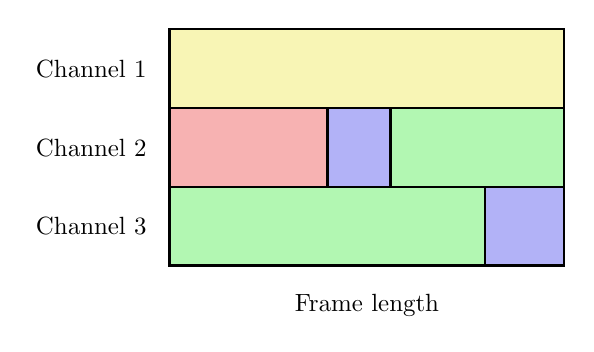
\begin{tikzpicture}
\draw[black,very thick] (-4,-1) rectangle (1,0);
\draw[black,very thick] (-4,0) rectangle (1,1);
\draw[black,very thick] (-4,1) rectangle (1,2);
\draw [step=.3, thick, draw= black, fill=black!10!green!30] (-4,-1) rectangle  (0,0);
\draw [step=.3, thick, draw= black, fill=black!10!blue!30] (0,-1) rectangle  (1,0);
\draw [step=.3, thick, draw= black, fill=black!10!red!30] (-4,0) rectangle  (-2,1);
\draw [step=.3, thick, draw= black, fill=black!10!blue!30] (-2,0) rectangle  (-1.2,1);
\draw [step=.3, thick, draw= black, fill=black!10!green!30] (-1.2,0) rectangle  (1,1);
\draw [step=.3, thick, draw= black, fill=black!10!yellow!30] (-4,1) rectangle  (1,2);
\node[align=center, scale =0.9] at (-1.5,-1.5) {Frame length};
\node[align=center, scale =0.9] at (-5,-.5) {Channel 3};
\node[align=center, scale =0.9] at (-5,.5) {Channel 2};
\node[align=center, scale =0.9] at (-5,1.5) {Channel 1};
\end{tikzpicture}

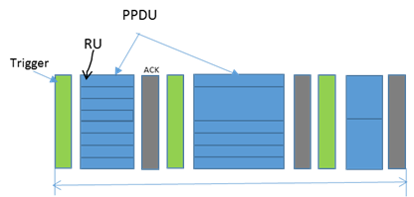
\includegraphics[width=0.5\textwidth]{../images/schedule2.png}
\caption{Multiplexing of frequencies (RU) and time (PPDU) in IEEE 802.11ax transmission window (formally referred as Transmission Opportunity or TXOP in the standard. The total transmission time is the time of all PPDUs, including the overhead of trigger frames (TF) and acknowledgments.}
\label{fig_multiplex}
\end{figure}
%%%%%%%%%%%%%%%%%%%%%

We consider the communication model provided in the next-generation Wi-Fi standard IEEE 802.11ax. While 3GPP wireless systems such as LTE~\cite{sesia2011lte} or the next generation 5G~\cite{agiwal2016next} can also be considered as alternate communication models, most factory floors are already equipped with Wi-Fi connectivity and, moreover, Wi-Fi can operate in the unlicensed band. It is generally considered to be cost-effective to operate and maintain.

Traditional Wi-Fi systems rely only on contention-based channel access and may introduce high or variable latency in congested or dense deployment scenarios even in a fully managed Wi-Fi network, which is typically available in industrial control and automation scenarios. To address the problems with dense deployment, the draft 802.11ax amendment has defined scheduling capability for Wi-Fi access points (APs). Wi-Fi devices can now be scheduled for accessing the channel in addition to the traditional contention-based channel access. Such scheduled access enables more controlled and deterministic behavior in the Wi-Fi networks. Within each transmission window (formally referred as transmission opportunity or TXOP in the standard), the AP may schedule devices through both frequency and time division multiplexing using the multi-user (MU) OFDMA technique. This to say that devices can be slotted in various frequency bands---formally called resource units (RUs)---and in different timed transmission slots---formally called PPDUs. An example of the multiplexing of devices across time and frequency is demonstrated in Figure \ref{fig_multiplex}. The AP additionally sends a trigger frame (TF) indicating which devices should transmit data in the current TXOP and the time/frequency resources these triggered devices should use in their transmissions. 

To state this model formally, the scheduling parameters assigned by the AP to each device consist of a frequency-slotted RU, time-slotted PPDU, and an associated modulation and coding scheme (MCS) to determine the transmission format. The transmission power is assumed to be fixed and equally divided amongst all devices. We define the following notations to formulate these parameters.  To specify an RU, we first notate by $f^1, f^2, \hdots, f^b$, where $n$ is the number of discrete frequency bands of fixed bandwidth (typically 2 MHz) in which a device can transmit; in a 20MHz channel, for example, there are $n=10$ such bands. For each device, we then define a set of binary variables $\varsigma^j_{i} \in \{0,1\}$ if device $i$ transmits in band $f^j$ and collect all such variables for device $i$ in $\bbsigma_i = [\varsigma^1_{i};\hdots;\varsigma^b_{i}] \in \{0,1\}^{b}$ and for all devices in  $\bbSigma := [\bbsigma_i, \hdots, \bbsigma_m] \in \{0,1\}^{b \times m}$. A device may transmit in bands in certain multiples of 2MHz as well, which would be notated as, e.g. $\bbsigma_i = [1; 1; 0; \hdots; 0]$ for transmission in an RU of size 4MHz. Note, however, that allowable RU's contain only sizes of certain multiples of 2MHz---namely, 2MHz, 4MHz, 8MHz, and 20MHz in the 802.11ax standard. Furthermore, it is only permissible to transmit in \emph{adjacent} bands, e.g. $f^{j}$ and $f^{j+1}$. We therefore define the set $\ccalS \subset \{0,1\}^{b}$ as the set of binary vectors that define permissible RUs and consider only $\bbsigma_i \in \ccalS$ for all devices $i$.  Finally, note that the RU assignment $\bb0 \in \ccalS$ signifies a device does not transmit in this particular transmission window.

%%%%%%% T A B L E %%%%%%%%%%%
\begin{table}
\begin{tabular}{ l | l | l | l  }
\hline
  $\mu$ & Modulation type & Coding rate & Data rate (Mb/s)  \\ \hline
  0 & BPSK & 1/2 & 4 \\
  1 & QPSK & 1/2 & 16 \\
  2 & QPSK & 3/4 & 24 \\
  3 & 16-QAM & 1/2 & 33 \\
  4 & 16-QAM & 3/4 & 49 \\
  5 & 64-QAM & 2/3 & 65 \\
  6 & 64-QAM & 3/4 & 73 \\
  7 & 64-QAM & 5/6 & 81 \\
  8 & 256-QAM & 3/4 & 98 \\
  9 & 256-QAM & 5/6 & 108 \\
  10 & 1024-QAM & 3/4 & 122 \\
  \hline  
\end{tabular}
\caption{Data rates for MCS configurations in IEEE 802.11ax for 20MHz channel. The modulation type and coding rate in the first 2 columns together specify a PDR function $q(\bbmu,\bbsigma)$ for RU $\bbsigma$. The data rate in the third column specifies the associated transmission time $\tau(\mu, \bbsigma)$. }
\label{tab_mcs}
\end{table}
%%%%%%%%%%%%%%%%%%%%%

To specify the PPDU of all scheduled devices, we define for device $i$ a positive integer value $\alpha_i \in \mathbb{Z}_{++}$ that denotes the PPDU slot in which it transmits and collect such variables for all devices in $\bbalpha = [\alpha_1; \hdots; \alpha_m] \in \mathbb{Z}_{++}^m$. Likewise, device $i$ is given an MCS $\mu_i$ from the discrete space $\ccalM = \{0,1,2,\hdots,10\}$. The MCS in particular defines a pair of modulation scheme and coding rate that subsequently determine both the data rate and packet error rate of the transmission. The allowable MCS settings provided in 802.11ax are provided in Table \ref{tab_mcs}. Finally, we notate by $\bbh_{i} := [h_i^1; h_i^2; \hdots; h_i^b] \in \reals^b_+$ a set of channel states experienced by device $i$, where $h_i^j$ is the gain of a wireless fading channel in frequency band $f^j$. We assume that channel conditions are constant within a single TXOP, i.e. do not vary across PPDUs.

We now proceed to define two functions that describe the wireless communications over the channel. Firstly, we define a function  $q: \reals_+^b \times \ccalM \times \ccalS \rightarrow [0,1]$ which, given a set of channel conditions $\bbh$, MCS $\mu$, and RU $\bbsigma$, returns the probability of successful transmission, otherwise called packet delivery rate (PDR). Furthermore, define by $\tau: \ccalM \times \ccalS  \rightarrow \reals_+$ a function that, given an MCS $\mu$ and RU $\bbsigma$, returns the maximum time taken for a single transmission attempt. Assuming a fixed packet size, such a function can be determined from the data rates associated with each MCS in Table \ref{tab_mcs}.  Observe that all functions just defined are determined independent of the PPDU slot the transmission takes place in, while transmission time is also independent of the channel state. Because a PPDU cannot finish until all transmissions within the PPDU have been completed, the total transmission time of a single PPDU $s$ is the maximum transmission time taken by all devices within that time slot. We define the transmission time of PPDU slot $s$ as
%
\begin{equation}\label{eq_time_slot}
\hat{\tau}(\bbSigma, \bbmu, \bbalpha, s) := \max_{i: \alpha_i = s} \tau(\mu_i, \bbsigma_i) + \tau_0(\bbalpha,s),
\end{equation}
%
where $\tau_0: \mathbb{Z}_{++}^m \times \mathbb{Z}_{++} \rightarrow \reals_+$ is a function that specifies the communication overhead of PPDU $s$. This overhead may consist of, e.g., the time required to send TFs to scheduled users, as seen in Figure \ref{fig_multiplex}.

%\begin{remark}\normalfont
%Note that, while in the next sections we proceed to derive the scheduling problem and method specifically for the IEEE 802.11ax standard, the concepts we discuss and overall approach can be applied generically to any communication standard that permits centralized resource allocation and scheduling, e.g., LTE. We discuss these details as they pertain to IEEE 802.11ax primarily for its applicability in industrial control settings, but a corresponding scheduling protocol for other standards can be immediately obtained by substituting the above scheduling parameters, e.g. RUs, MCS, etc., with the available parameters for the communication standard of interest.
%\end{remark}
